\chapter{پیاده‌سازی و کتابخانه‌ها}

\section{مقدمه}
در این قسمت قصد داریم بخش پیاده‌سازی و کتابخانه‌های استفاده ‌شده را توضیح دهیم. پروژه با زبان برنامه‌نویسی پایتون پیاده‌سازی شده است. با توجه به معماری مدل‌های مبتنی بر شبکه‌های عصبی بازگشتی، برای پردازش با سرعت مناسب بهتر بود از پردازنده‌های گرافیکی\LTRfootnote{\lr{Graphics Processing Unit}} استفاده کنیم. به همین منظور، تمام کدهای پروژه بر روی سرویس کولب\LTRfootnote{\lr{Google Colaboratory}}، که به صورت رایگان امکان استفاده از پردازنده‌های گرافیکی به کاربران می‌دهد، اجرا شده است. در ادامه این بخش به تشریح قسمت‌های مختلف پیاده‌سازی و کتابخانه‌های استفاده ‌شده می‌پردازیم.

\section{واکشی و پیش‌پردازش دفتر ثبت سفارشات}
در این قسمت ابتدا نحوه‌ی واکشی اطلاعات دفتر ثبت سفارشات از صرافی آنلاین بایننس\LTRfootnote{Binance} به وسیله کتابخانه‌ی سی‌سی‌ایکس‌تی\LTRfootnote{ccxt} را تشریح می‌کنیم. سپس به نحوه‌ی ذخیره‌سازی سری‌های زمانی و ساخت مجموعه داده برچسب خورده برای یادگیری می‌پردازیم. در انتها نیز پیاده سازی مدل جی‌آريو و یادگیری مدل و تابع خطا را تشریح می‌کنیم.
\subsection{واکشی دفتر ثبت سفارشات}
هر رمز ارز در هر صرافی دارای دفتر سفارشات مخصوص به خود است. این دفاتر شامل سفارش‌های از جنس آن رمز ارز در آن صرافی هستند که بنا به سیاست هر صرافی می‌توان تاریخچه‌ی آن‌ها را درخواست کرد و مورد مطالعه قرار داد. در اینجا ما از داده‌های دفتر ثبت سفارشات صرافی بایننس که هم‌اکنون بزرگترین صرافی رمزارزها در دنیاست استفاده می‌کنیم. صرافی بایننس اجازه‌ی واکشی اطلاعات مربوط به دفتر سفارشات رمزارزهای گوناگونی که در آن مبادله می‌شوند را به کاربران خود می‌دهد که ما در این میان به مطالعه‌ی پنج رمزارز بزرگ‌تر می‌پردازیم.
\newpage
رمزارزهای مورد مطالعه:
\begin{itemize}
	\item بیتکوین\LTRfootnote{Bitcoin}
	\item اتریوم\LTRfootnote{Ethereum}
	\item بایننس کوین\LTRfootnote{Binance Coin}
	\item کاردانو\LTRfootnote{Cardano}
	\item دوج کوین\LTRfootnote{Doge Coin}
\end{itemize}
 اطلاعات مربوط به دفتر سفارشات این رمزارزها در صرافی بایننس و در بازه‌ی زمانی ابتدای ۲۰۲۰ تا ابتدای ۲۰۲۱ در این پروژه به کار گرفته شده است. برای واکشی اطلاعات مربوط به این رمزارز‌ها از کتابخانه‌ی سی‌سی‌ایکس‌تی\LTRfootnote{https://github.com/ccxt/ccxt} که یک کتابخانه‌ی مخصوص برای مطالعه و خرید و فروش رمز ارزهاست استفاده شده است.\\
 اطلاعات مربوط به هر رمزارز به صورت مجموعه‌ای از دفترهای سفارش در طول زمان و با فاصله‌ی زمانی یک دقیقه‌ای جمع‌آوری شده‌ است این دفترها که هرکدام موجودیتی سه‌بعدی هستند(شکل \ref{fig.orderbook_structure}) در طول زمان کنار یکدیگر قرار می‌گیرند و درنهایت یک آرایه‌ی چهاربعدی تشکیل می‌دهند. اما همانطور که پیش‌تر گفته شد این دفترها ابتدا به دفترهای سفارش تجمعی تبدیل می‌شوند و سپس قیمت میانی از آن‌ها استخراج می‌شود. به همین دلیل در ادامه، دیگر نیازی به دندانه‌های قیمت نخواهد بود چرا که فاصله‌ی آن‌ها توسط صرافی برابر مقدار ثابتی از مقدار میانی درنظر گرفته می‌شود و به همین دلیل نیازی به ذخیره‌سازی و وارد کردن این دندانه‌های با طول ثابت به مدل شبکه‌ی عصبی وجود نخواهد داشت. بر این اساس، با حذف دندانه‌های قیمت و ذخیره‌سازی حجم‌های متناظر مجموعه‌داده‌ی ورودی را تشکیل می‌دهیم.\\
 از طرف دیگر ویژگی‌هایی که در قسمت روش حل مسئله به آن‌ها اشاره کردیم را به مجموعه‌داده اضافه می‌کنیم که شامل قیمت میانی،
  شکاف قیمت، تغییر قیمت(بازده)، شکاف قیمت وزن‌دار و نوسان با دامنه‌های متفاوت است.\\
\begin{figure}[!t]
	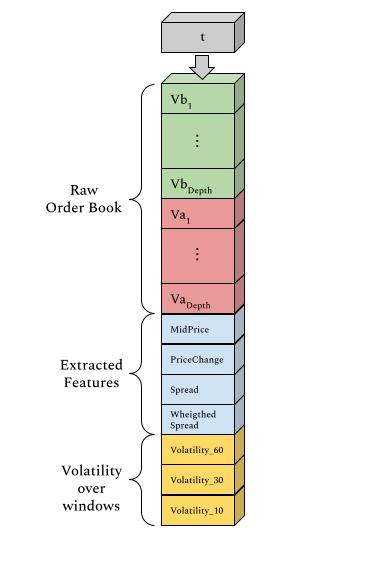
\includegraphics[width=0.5 \textwidth]{images/dataset_1}
	\centering
	\caption{اطلاعات ورودی به ازای هر لحظه‌ي $t$ در طول زمان	}
	\label{fig.dataset_1}
\end{figure}
بدین ترتیب در هر نقطه‌ از زمان مجموعه‌ای از اطلاعات جمع‌آوری و محاسبه می‌شود که می‌تواند برای یادگیری استفاده شود. در ادامه می‌توانیم با کنار هم قرار دادن دنباله‌ای از ستون‌هایی ازین جنس به یک یک ماتریس دست پیدا کنیم که هر ستون آن می‌تواند به یکی از واحد‌های مدل‌ جی‌آریو به عنوان ورودی داده شود.\\
هر دنباله‌ی ورودی که خود شامل تعدادی از ستون‌های شکل \ref{fig.dataset_1} است، می‌تواند توسط یک عدد که میزان نوسان در دقیقه‌ی آینده و یا پنج دقیقه‌ی آینده‌ی بعد از آن برچسب بخورد و برای آموزش به مدل داده شود. بنابراین نحوه‌ي برچسب‌زنی مجموعه‌ی نهایی به سه متغیر طول پنجره‌ی ورودی، حاشیه\LTRfootnote{Offset} و طول پنجره‌ی پیش‌بینی بستگی خواهد داشت(شکل \ref{fig.input_gru}).
\newpage
\begin{figure}[!t]
	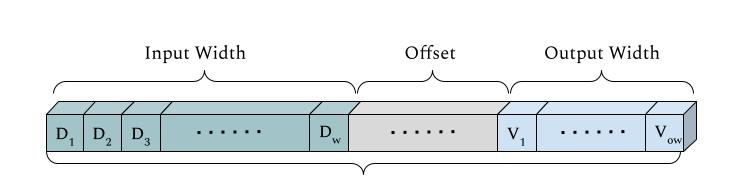
\includegraphics[width=1 \textwidth]{images/input_gru}
	\centering
	\caption{اطلاعات ورودی به ازای هر لحظه‌ي $t$ در طول زمان	}
	\label{fig.input_gru}
\end{figure}
به این صورت مجموعه‌داده نهایی به صورت مجموعه‌ای دنباله‌های ورودی با طول مشخص و برابر $W$ و خروجی متناظر با نوسان در بازه‌ای در آینده با طول $OW$ خواهد بود. طبیعی است که این مقادیر بسته به هدف استفاده از‌ مدل و توانایی پردازشی سیستم تعیین می‌شوند.
\section{مدل و یادگیری}
برای پیاده سازی مدل جی‌آریو از کتاب‌خانه‌ی تنسورفلو\LTRfootnote{Tensorflow} استفاده کرده‌ایم. این کتابخانه که مخصوص طراحی و آموزش شبکه‌های عصبی است، شامل پیاده‌سازی انواع مختلفی از شبکه‌های عصبیست که باعث شده در سال‌های گذشته به طور گسترده به کار گرفته شود.\\
\begin{figure}[!t]
	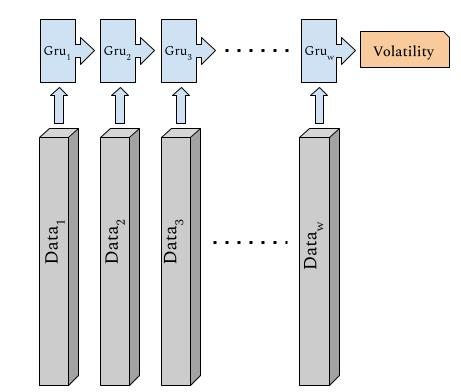
\includegraphics[width=0.6 \textwidth]{images/gru_function}
	\centering
	\caption{واردشدن اطلاعات ورودی به جی‌آریو برای تخمین نوسان}
	\label{fig.gru_function}
\end{figure}
\newpage
اطلاعات بدست آمده در مرحله‌ی قبل مانند شکل \ref{fig.gru_function} به عنوان ورودی به جی‌آریو داده می‌شوند و درنهایت به وسیله‌ی خطای محاسبه‌ شده آموزش داده می‌شود.
\section{جمع‌بندی}
در این فصل کتابخانه‌های استفاده شده را معرفی کردیم و به بیان جزییات ساخت مجموعه داده مورد استفاده پرداختیم. در ادامه به پیاده سازی شبکه‌ی عصبی جی‌آریو و نحوه‌ی انجام عمل یادگیری به وسیله‌ی داده‌های برچسب خورده پرداختیم.






